\begin{center}
    {\large\bfseries 6 класс. Занятие 1. Ответы}
\end{center}

\footnotesize

\begin{enumerate}[itemsep=0.7em]

\item
\begin{enumerate}[label={},leftmargin=1.7em,itemsep=0.35em]
\item[а)] Верно.
\item[б)] Неверно: $3^2$ делится на $9$, но $3$ не делится на $9$.
\item[в)] Неверно: например, неквадратный прямоугольник со сторонами $2$ и $3$.
\item[г)] Для произвольных чисел неверно: например, $12{,}5>12$, но
$12{,}5<13$. Для целых чисел утверждение верно.
\item[д)] Неверно: треугольник тоже можно одним разрезом разделить на два
треугольника.
\end{enumerate}

\item Направления стрелок:
\begin{enumerate}[label={},leftmargin=1.7em,itemsep=0.35em]
\item[а)] оканчивается цифрой $0\ \Longleftrightarrow\ $ делится на $10$;
\item[б)] делится на $15\ \Longrightarrow\ $ делится на $5$;
\item[в)] квадрат $\Longrightarrow$ ромб;
\item[г)] $ab$ делится на $6\ \Longleftarrow\ a$ или $b$ делится на $6$;
\item[д)] $n^2$ делится на $12\ \Longleftrightarrow\ n$ делится на $6$.
\end{enumerate}

\item 1) следует; \quad 2) не следует; \quad 3) следует; \quad
4) следует; \quad 5) следует; \quad 6) не следует.

Для пункта 2 биолог может носить белый бейдж. Для пункта 6 контрпримером
может быть биолог с белым бейджем, который не работает в лаборатории №~5.

\item Контрпримеры:
\begin{enumerate}[label={},leftmargin=1.7em,itemsep=0.35em]
\item[а)] $2+3=5$ --- простое число;
\item[б)] прямоугольники $1\times10$ и $4\times4$: $22>16$, но $10<16$;
\item[в)] $\dfrac21>\dfrac32$, то есть после прибавления $1$ к числителю
и знаменателю дробь уменьшилась.
\end{enumerate}

\item $x=9$.

\end{enumerate}

\newpage

\begin{center}
    {\large\bfseries Непрерывная олимпиада. Тур 1. Ответы}
\end{center}

\small

\begin{enumerate}[itemsep=1em]

\item $9876432150$.

\item Один из вариантов разрезания:

\begin{center}
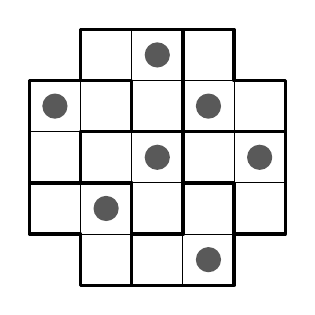
\begin{tikzpicture}[x=0.65cm,y=0.65cm,line join=round]
    \foreach \x in {1,2,3} {
        \draw[line width=0.35pt] (\x,0) rectangle ++(1,-1);
        \draw[line width=0.35pt] (\x,-4) rectangle ++(1,-1);
    }
    \foreach \y in {-1,-2,-3} {
        \foreach \x in {0,1,2,3,4} {
            \draw[line width=0.35pt] (\x,\y) rectangle ++(1,-1);
        }
    }

    \draw[line width=1.2pt] (1,0)--(3,0)--(3,-2)--(2,-2)--(2,-1)--(1,-1)--cycle;
    \draw[line width=1.2pt] (3,0)--(4,0)--(4,-1)--(5,-1)--(5,-2)--(3,-2)--cycle;
    \draw[line width=1.2pt] (0,-1)--(2,-1)--(2,-2)--(1,-2)--(1,-3)--(0,-3)--cycle;
    \draw[line width=1.2pt] (1,-2)--(3,-2)--(3,-4)--(2,-4)--(2,-3)--(1,-3)--cycle;
    \draw[line width=1.2pt] (3,-2)--(5,-2)--(5,-4)--(4,-4)--(4,-3)--(3,-3)--cycle;
    \draw[line width=1.2pt] (0,-3)--(2,-3)--(2,-5)--(1,-5)--(1,-4)--(0,-4)--cycle;
    \draw[line width=1.2pt] (3,-3)--(4,-3)--(4,-5)--(2,-5)--(2,-4)--(3,-4)--cycle;

    \foreach \p in {(2.5,-0.5),(0.5,-1.5),(3.5,-1.5),
                     (2.5,-2.5),(4.5,-2.5),(1.5,-3.5),(3.5,-4.5)} {
        \fill[black!65] \p circle[radius=0.16cm];
    }
\end{tikzpicture}
\end{center}

\item $27$ кг. Например, веса дынь могут быть
$1$, $2$, $6$, $7$ и $11$ кг.

\end{enumerate}
